%\documentclass[10pt]{article}
%\usepackage[utf8]{inputenc}
%\usepackage[T1]{fontenc}
%\usepackage{graphicx}
%\usepackage[export]{adjustbox}
%\graphicspath{ {./images/} }
%\usepackage{amsmath}
%\usepackage{amsfonts}
%\usepackage{amssymb}
%\usepackage[version=4]{mhchem}
%\usepackage{stmaryrd}
%
%\title{Contexte }
%
%%\author{}
%%\date{}
%
%
%\begin{document}
%\maketitle
%\begin{center}
%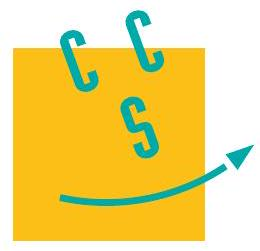
\includegraphics[width=\textwidth]{2023_07_26_54f5e859400a10e656ddg-01}
%\end{center}

\section*{Contexte}
Les recours aux opérations chirurgicales pour traiter les pathologies cardiaques sont de plus en plus courants. La plupart de ces opérations est actuellement réalisée après avoir arrêté le cœur du patient et mis en place une circulation et une oxygénation extérieures du sang. Cette procédure et les suites opératoires sont lourdes.

Il est possible d'opérer sans arrêter le cœur, mais ce type d'opération à cœur battant est plus délicat pour le chirurgien à cause des mouvements de la zone à opérer dûs à la respiration et aux battements du cœur. Les battements cardiaques, contrairement aux mouvements respiratoires, ne sont pas cycliques et engendrent un déplacement rapide de la zone à opérer. Une intervention robotisée type maitre-esclave avec prise en compte des battements cardiaques pour le déplacement du robot esclave est compliquée et dangereuse.

Lors d'une opération à cœur battant, un maintien mécanique de la zone à opérer est indispensable. Ce maintien en position est réalisé par un stabilisateur composé de deux doigts en contact avec la zone à opérer. Le déplacement de la zone à opérer est ainsi diminué. Le stabilisateur est lié à la table d'opération par une attache reconfigurable. La stabilisation (\autoref{fig_ccspsi2022:01}) peut être active ou passive. Dans le cas d'une stabilisation active, un actionneur génère une action mécanique de compensation dans le but de diminuer le mouvement de la zone à opérer qui n'a pas été filtré par le stabilisateur passif. Ce mouvement constitue un déplacement résiduel.
\begin{figure}[!h]
\centering
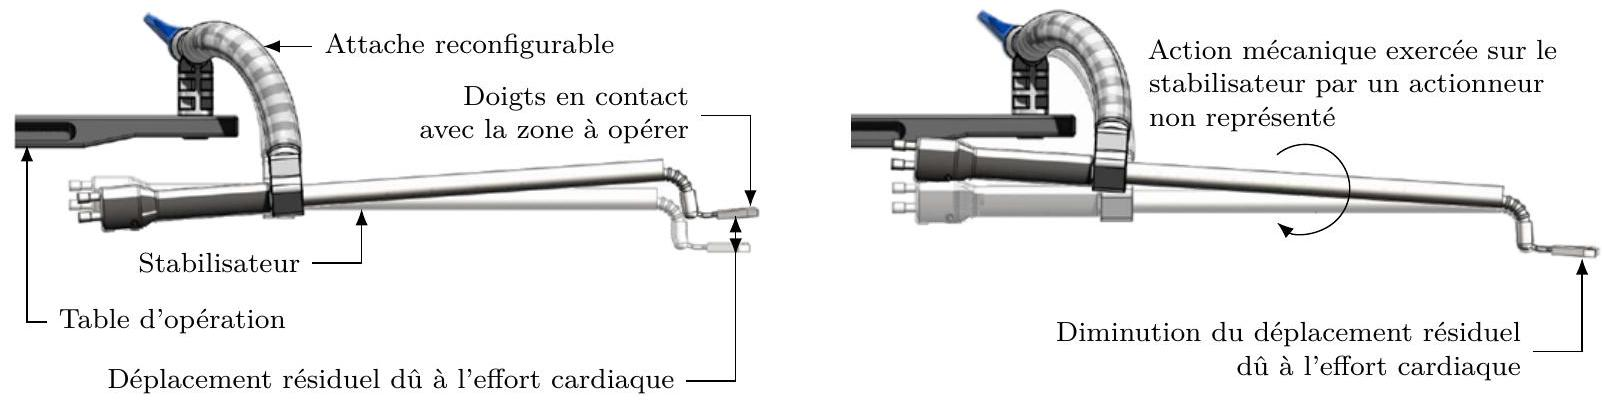
\includegraphics[width=\textwidth]{2023_07_26_54f5e859400a10e656ddg-01(1)}
\caption{Stabilisations passive (à gauche) et active (à droite) \label{fig_ccspsi2022:01}}
%Figure 1 
\end{figure}

Une équipe de chercheurs de l'Université de Strasbourg a mis au point un dispositif utilisant l'effet gyroscopique (\autoref{fig_ccspsi2022:02}).

\begin{figure}[!h]
\centering
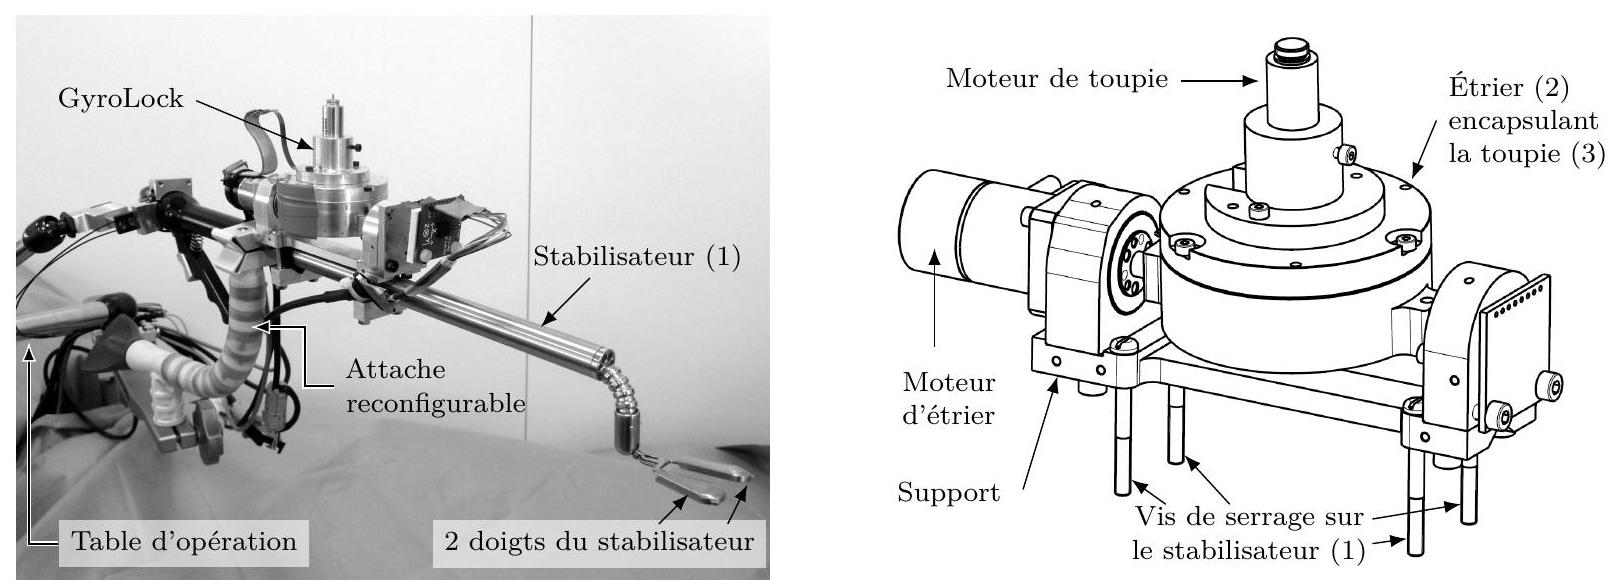
\includegraphics[width=\textwidth]{2023_07_26_54f5e859400a10e656ddg-01(2)}
%Figure 2 
\caption{\label{fig_ccspsi2022:02}Photo du GyroLock installé sur un stabilisateur (à gauche) et son modèle volumique (à droite)}
\end{figure}


Ce système, nommé GyroLock, présente deux avantages par rapport aux autres stabilisateurs actifs existants :

\begin{itemize}
  \item il peut être mis en place sur la plupart des stabilisateurs passifs afin de limiter l'investissement financier des structures hospitalières voulant s'équiper de stabilisateurs actifs ;

  \item il ne nécessite pas de liaison avec la table d'opération donc le stabilisateur peut être placé dans n'importe quelle position. En effet, contrairement aux autres stabilisateurs actifs existants, le GyroLock ne comporte pas d'actionneur dont le stator est lié à la table d'opération.

\end{itemize}

Le GyroLock est muni de deux actionneurs. Le moteur de toupie met en rotation la toupie (3) par rapport à l'étrier (2) autour d'un axe initialement vertical. Un second moteur électrique, appelé moteur d'étrier, entraine en rotation l'étrier (2) par rapport au support lié au stabilisateur (1) autour d'un axe colinéaire à la direction du stabilisateur (1). Cette seconde rotation génère un effet dynamique appelé effet gyroscopique. Cet effet peut être considéré comme une action mécanique permettant d'atténuer le déplacement résiduel de la zone à opérer en contact avec les doigts du stabilisateur (1).

\subsection*{Exigences fonctionnelles}
Le diagramme des exigences partiel de la stabilisation cardiaque est donné \autoref{fig_ccspsi2022:03}.


\begin{figure}[!h]
\centering
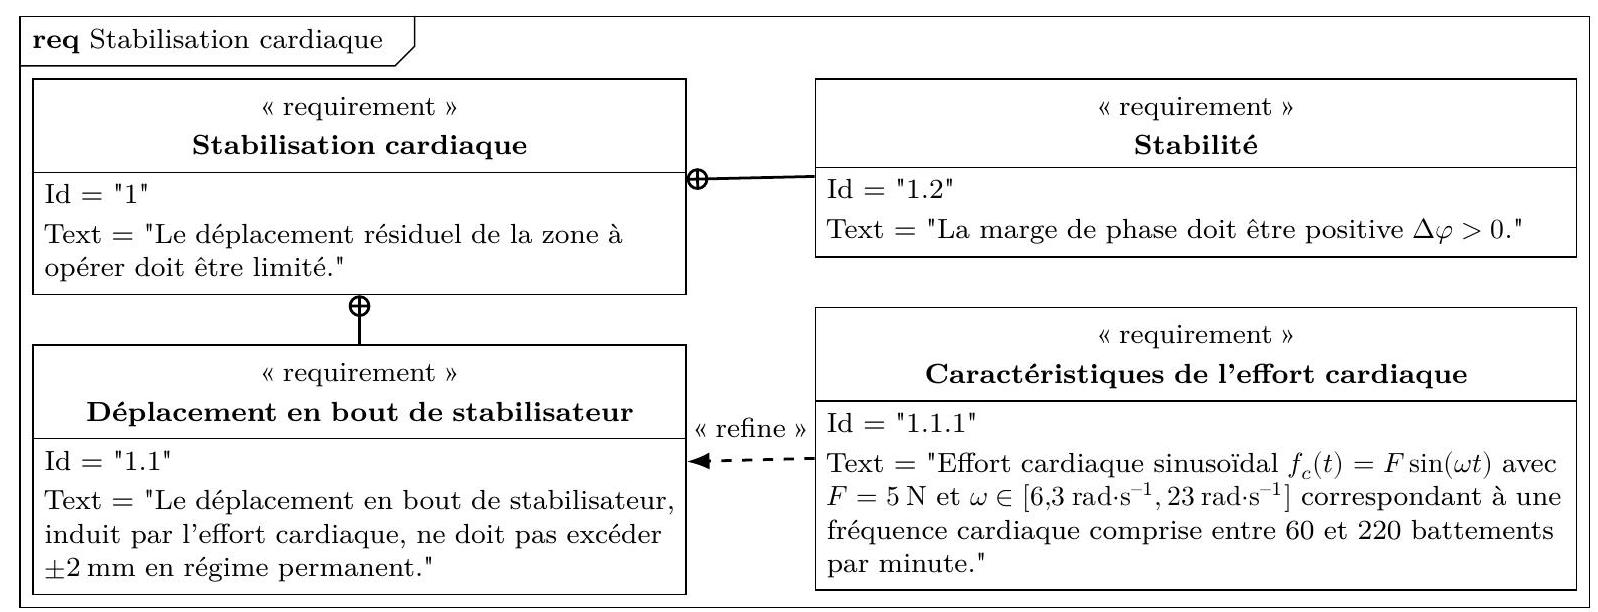
\includegraphics[width=\textwidth]{2023_07_26_54f5e859400a10e656ddg-02(1)}
% Figure 3 
\caption{Diagramme des exigences partiel\label{fig_ccspsi2022:03}}
\end{figure}

\begin{obj}
L'objectif de ce sujet est de montrer que l'utilisation d'un actionneur à effet gyroscopique permet d'améliorer le maintien de la zone à opérer. Les étapes nécessaires à la validation de cet objectif sont les suivantes :
\end{obj}

\begin{itemize}
  \item dans un premier temps, l'analyse de résultats expérimentaux permettra de modéliser le mécanisme ;

  \item après avoir analysé l'effet gyroscopique et réglé le correcteur empêchant la dérive de l'étrier, une étude dynamique du stabilisateur permettra de déterminer un modèle de comportement du stabilisateur ;

  \item enfin, la partie III traitera du choix d'une loi de commande permettant de respecter les exigences figure \ref{fig_ccspsi2022:03}.

\end{itemize}

\section{Résultats expérimentaux et modélisation du mécanisme}
\begin{obj}
Exploiter les résultats d'une campagne expérimentale afin de modéliser la liaison entre la table d'opération et le stabilisateur, puis exprimer le déplacement en bout de stabilisateur.
\end{obj}

\subsection{\label{sec:I.A} Mesure du déplacement en bout de stabilisateur}
Un stabilisateur passif (sans système de stabilisation active) a été testé sur un sujet porcin de $40 \mathrm{~kg}$ sous assistance respiratoire et anesthésie générale. Les volume et fréquence respiratoires sont respectivement de $300 \mathrm{~mL}$ et 15,6 respirations par minute. Une mesure du déplacement et de l'effort cardiaque au bout du stabilisateur passif a été effectuée.

Le système cardiovasculaire porcin étant similaire à celui d'un être humain, il est possible, grâce à une méthode non détaillée dans cette étude, d'estimer les valeurs équivalentes pour un homme de $90 \mathrm{~kg}$. La figure \ref{fig_ccspsi2022:04} donne l'évolution temporelle, pour un patient humain, du déplacement du point $P$ situé au bout du stabilisateur (figure~\ref{fig_ccspsi2022:05}).

\begin{figure}[!h]
\centering
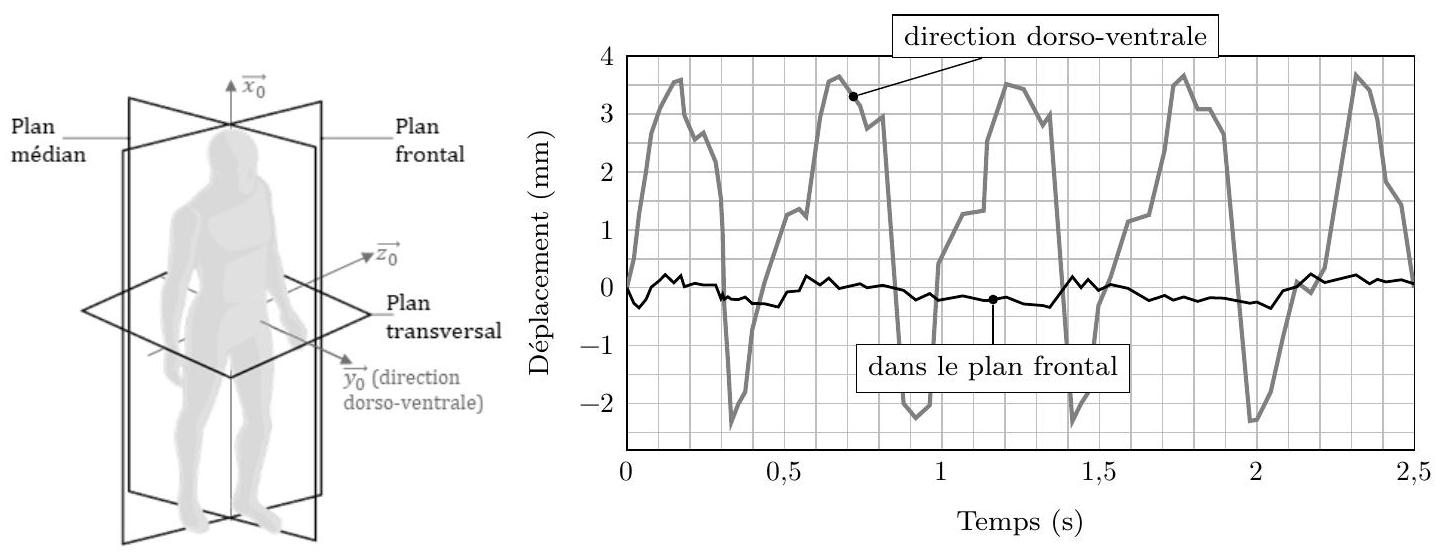
\includegraphics[width=\textwidth]{2023_07_26_54f5e859400a10e656ddg-02}
%Figure 4 
\caption{Plans anatomiques, déplacements résiduels dans le plan frontal et dans la direction dorso-ventrale\label{fig_ccspsi2022:04}}
\end{figure}


\question{Déterminer, à partir de la figure \ref{fig_ccspsi2022:04}, les valeurs minimales et maximales de déplacement du point $P$ dans la direction dorso-ventrale, notées $u_{d}^{\max }$ et $u_{d}^{\min }$, et dans le plan frontal, notées $u_{f}^{\max }$ et $u_{f}^{\min }$. Déterminer laquelle des deux stabilisations (passive ou active) est nécessaire pour respecter le diagramme des exigences figure \ref{fig_ccspsi2022:03}.}

La liaison entre le stabilisateur (1) et la table d'opération (0) sera modélisée de trois façons différentes selon la finalité :

\begin{itemize}
  \item par une liaison sphérique (partie \ref{sec:IB}) afin de déterminer quelles rotations doivent être prises en compte pour représenter le mouvement du stabilisateur par rapport à la table d'opération ;
  \item par un encastrement (partie \label{sec:IIA}) afin d'étudier l'effet gyroscopique sans prendre en compte le mouvement du stabilisateur ;
  \item par une liaison non parfaite (partie \label{sec:IIC}) modélisant la flexibilité de l'attache reconfigurable.
\end{itemize}

%% I.B
\subsection{\label{sec:I.B}Formulation du modèle de la liaison entre la table d'opération et le stabilisateur}
La modélisation retenue pour estimer le déplacement du point $P$ situé au bout du stabilisateur (1) est donnée figure \ref{fig_ccspsi2022:05}. La direction $\vec{y}_{0}$ correspond à la direction dorso-ventrale, le plan $\left(O_{0}, \vec{z}_{0}, \vec{x}_{0}\right)$ est le plan frontal et l'axe «pied-tête » du patient est représenté par le vecteur $\vec{x}_{0}$. Le point $O_{0}$ est un point de référence choisi, considéré comme fixe par rapport à la table d'opération (0).

\begin{figure}[!h]
\centering
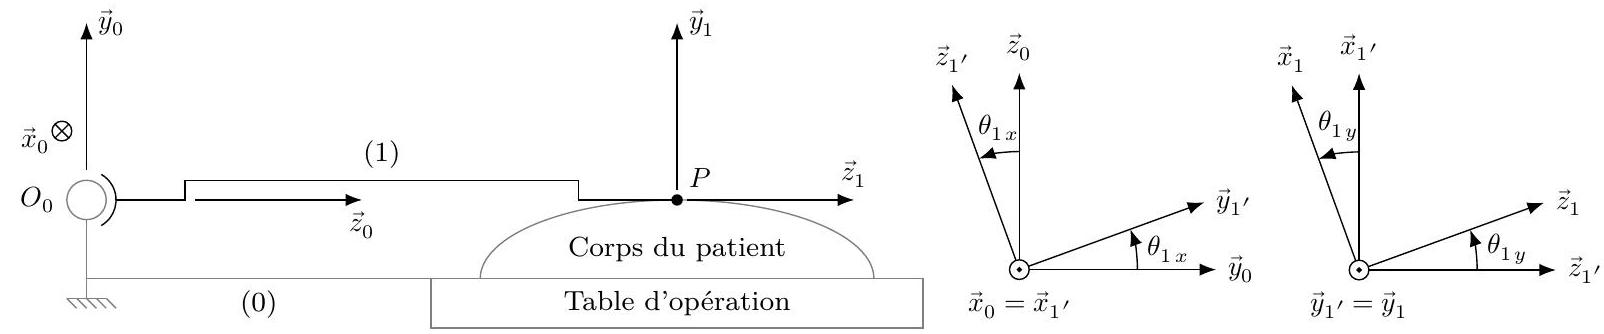
\includegraphics[width=\textwidth]{2023_07_26_54f5e859400a10e656ddg-03}
%Figure 5 
\caption{Modélisation du stabilisateur (1) en position de référence $\left(\theta_{1 x}=\theta_{1 y}=0\right)$ et figures de changement de base\label{fig_ccspsi2022:05}}
\end{figure}


Le déplacement du point $P$ situé au bout du stabilisateur (1) correspond à une trop grande flexibilité de l'attache reconfigurable (figures \label{fig_ccspsi2022:01} et \label{fig_ccspsi2022:02}) utilisée pour lier le stabilisateur à la table d'opération (0). La liaison entre les solides (0) et (1) est modélisée par une liaison sphérique de centre $O_{0}$.

Deux rotations successives permettent de positionner la base $\mathcal{B}_{1}\left(\vec{x}_{1}, \vec{y}_{1}, \vec{z}_{1}\right)$ liée au stabilisateur par rapport à la base $\mathcal{B}_{0}\left(\vec{x}_{0}, \vec{y}_{0}, \vec{z}_{0}\right)$ liée à la table d'opération :
\begin{itemize}
\item une rotation autour de $\vec{x}_{0}$ d'angle $\theta_{1 x}$ permet de définir une base intermédiaire $\mathcal{B}_{1}^{\prime}\left(\vec{x}_{0}, \vec{y}_{1^{\prime}}, \vec{z}_{1^{\prime}}\right)$;
\item une rotation autour de $\vec{y}_{1^{\prime}}$ d'angle $\theta_{1 \text { y }}$ permet d'orienter la base $\mathcal{B}_{1}$ par rapport à la base $\mathcal{B}_{1}^{\prime}$.
\end{itemize}

Les figures de changement de base sont données figure \label{fig_ccspsi2022:05}. La position du point $P$ par rapport à la table d'opération (0) est donnée par $\overrightarrow{O_{0} P}=L \vec{z}_{1}$ avec $L=0,3 \mathrm{~m}$. Le point $P_{0}$ tel que $\overrightarrow{O_{0} P_{0}}=L \vec{z}_{0}$ correspond à la position de référence du point $P$ pour laquelle $\theta_{1 x}=\theta_{1 y}=0$.

%Q 2. 
\question{\label{q:02}Exprimer le vecteur $\overrightarrow{P_{0} P}$ dans la base $\mathcal{B}_{0}$. En déduire l'expression de $u_{d}=\vec{P}_{0} P \cdot \vec{y}_{0}$ correspondant au déplacement en bout de stabilisateur dans la direction dorso-ventrale et $u_{f}=\left\|\overrightarrow{P_{0} P}-u_{d} \vec{y}_{0}\right\|$ traduisant le déplacement en bout de stabilisateur dans le plan frontal.}


%Q 3. 
\question{\label{q:03}Déterminer les expressions linéarisées à l'ordre 1 de $u_{d}$ et $u_{f}\left(\theta_{1 x}\right.$ et $\theta_{1 y}$ sont proches de 0$)$. En utilisant le résultat de la question 1, donner la valeur numérique (en radian) des débattements angulaires $\Delta \theta_{1 x}=$ $\max \left(\theta_{1 x}\right)-\min \left(\theta_{1 x}\right)$ et $\Delta \theta_{1 y}$ du stabilisateur. En déduire qu'une rotation peut être négligée (en précisant laquelle). En supposant que la rotation d'axe $\left(O_{0}, \vec{z}_{0}\right)$ est également négligeable, proposer une « nouvelle » liaison (en précisant ses caractéristiques géométriques) modélisant le mouvement du stabilisateur (1) par rapport à la table d'opération (0).}


%Q 4. 
\question{\label{q:04}Préciser alors la direction du moment de compensation que devra générer le système GyroLock afin de réduire le déplacement du point $P$.}

\section{Effet gyroscopique et modélisation du stabilisateur}
%\section{— Objectif}
\begin{obj}
Étudier les actions mécaniques créées par le système GyroLock, définir et régler la chaine d'asservissement de l'étrier puis modéliser le comportement du stabilisateur grâce à une étude dynamique.
\end{obj}

\subsection{\label{sec:IIA} Étude de l'effet gyroscopique généré par le système GyroLock}
Pour déterminer les actions mécaniques créées par le système GyroLock sur le stabilisateur (1), un modèle simplifié du mécanisme, donné figure \ref{fig_ccspsi2022:06}, est utilisé. Ce modèle simplifié, dans lequel la liaison entre le stabilisateur (1) et la table d'opération (0) est modélisée par un encastrement, permet :

\begin{itemize}
  \item d'étudier l'effet gyroscopique $c_{x}(t)$ créé par le système GyroLock permettant de compenser l'effet de l'effort cardiaque, sans prendre en compte le mouvement du stabilisateur (1);

  \item de déterminer les conditions d'utilisation du système GyroLock afin de minimiser les autres actions mécaniques créées et considérées comme indésirables.
\end{itemize}


\begin{figure}[!h]
\centering
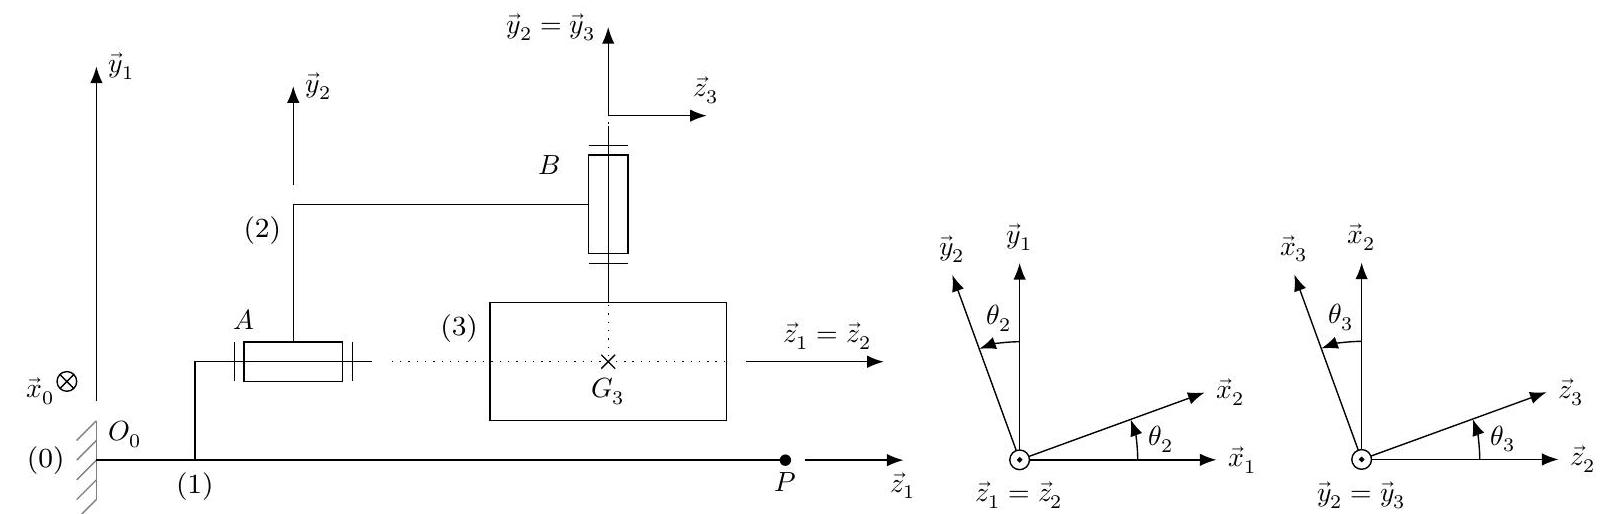
\includegraphics[width=\textwidth]{2023_07_26_54f5e859400a10e656ddg-04}
%Figure 6 
\caption{\label{fig_ccspsi2022:06}Schéma cinématique simplifié du mécanisme (représenté pour $\theta_{2}=\theta_{3}=0$ ) et figures de changement de base}
\end{figure}

%
%Le système GyroLock, dont la modélisation est donnée figure \ref{fig_ccspsi2022:06}, est composé de trois solides :
%
%\begin{itemize}
%  \item le support, relié au stabilisateur (1) de repère associé $\mathcal{R}_{1}\left(O_{0}, \vec{x}_{1}, \vec{y}_{1}, \vec{z}_{1}\right)$, en liaison encastrement au point $O_{0}$ avec la table d'opération $(0)$;
%
%  \item l'étrier (2) de repère associé $\mathcal{R}_{2}\left(A, \vec{x}_{2}, \vec{y}_{2}, \vec{z}_{1}=\vec{z}_{2}\right)$ tel que $\theta_{2}=\left(\vec{x}_{1}, \vec{x}_{2}\right)=\left(\vec{y}_{1}, \vec{y}_{2}\right)$;
%
%  \item la toupie (3) de repère associé $\mathcal{R}_{3}\left(B, \vec{x}_{3}, \vec{y}_{2}=\vec{y}_{3}, \vec{z}_{3}\right)$ tel que $\theta_{3}=\left(\vec{x}_{2}, \vec{x}_{3}\right)=\left(\vec{z}_{2}, \vec{z}_{3}\right)$.
%
%\end{itemize}
%
%Les figures de changement de base sont données figure \ref{fig_ccspsi2022:06}. Toutes les liaisons sont supposées parfaites et les caractéristiques inertielles des solides sont les suivantes :
%\begin{itemize}
%\item étrier (2) : masse et inertie négligeables ;
%\item toupie (3) : masse $m_{3}$, centre d'inertie $G_{3}$ tel que $\overrightarrow{O_{0} G_{3}}=L_{G_{3}} \vec{z}_{1}+H_{G_{3}} \vec{y}_{1}$. L'axe $\left(G_{3}, \vec{y}_{3}=\vec{y}_{2}\right)$ étant un axe de symétrie de révolution de la toupie (3), sa matrice d'inertie au point $G_{3}$ s'exprime dans la base $\mathcal{B}_{2}$ sous la forme $\mathcal{J}\left(G_{3}, 3\right)=\left[\begin{array}{ccc}A_{3} & 0 & 0 \\ 0 & B_{3} & 0 \\ 0 & 0 & A_{3}\end{array}\right]_{\mathcal{B}_{2}}$.
%\end{itemize}
%
%Pour la modélisation des actions mécaniques extérieures, les hypothèses suivantes sont adoptées :
%
%\begin{itemize}
%  \item les actions mécaniques dues à la pesanteur sont négligées devant les effets dynamiques ;
%
%  \item l'action mécanique transmise par la liaison encastrement entre les solides (0) et (1) est modélisée au point $G_{3} \operatorname{par}\left\{\mathcal{T}_{0 \rightarrow 1}\right\}=\left\{\begin{array}{c}X_{01} \vec{x}_{1}+Y_{01} \vec{y}_{1}+Z_{01} \vec{z}_{1} \\ L_{01} \vec{x}_{1}+M_{01} \vec{y}_{1}+N_{01} \vec{z}_{1}\end{array}\right\}_{G_{3}}$.
%
%\end{itemize}
%
%Le référentiel $\mathcal{R}_{0}\left(O_{0}, \vec{x}_{0}, \vec{y}_{0}, \vec{z}_{0}\right)$ lié à la table d'opération (0) est galiléen.
%
%%Q 5.
%\question{\label{q:05} Exprimer, dans la base $\mathcal{B}_{2}$, le moment cinétique au point $G_{3}$ du solide (3) en mouvement dans le référentiel $\mathcal{R}_{0}$, noté $\vec{\sigma}\left(G_{3}, 3 / 0\right)$.}
%
%%Q 6. 
%\question{\label{q:06}En déduire, dans la base $\mathcal{B}_{2}$, le moment dynamique au point $G_{3}$ du solide (3) en mouvement dans le référentiel $\mathcal{R}_{0}$, noté $\vec{\delta}\left(G_{3}, 3 / 0\right)$.}
%
%%Q 7. 
%\question{\label{q:07}Après avoir clairement précisé le système isolé et le théorème utilisé, exprimer $L_{01}, M_{01}$ et $N_{01}$ en fonction de $\theta_{2}, \theta_{3}$ (et leurs dérivées temporelles), $A_{3}$ et $B_{3}$.}
%
%Lorsque la toupie (3) tourne avec une vitesse constante $\omega_{3}$ par rapport à l'étrier (2), l'expression des moments $L_{01}, M_{01}$ et $N_{01}$ est la suivante :
%
%$$
%\left\{\begin{array}{l}
%L_{01}(t)=-c_{x}(t) \cos \theta_{2}(t) \\
%M_{01}(t)=-c_{x}(t) \sin \theta_{2}(t) \\
%N_{01}(t)=A_{3} \ddot{\theta}_{2}(t)
%\end{array}\right.
%$$
%
%où $c_{x}(t)=B_{3} \omega_{3} \dot{\theta}_{2}(t)=K_{3} \dot{\theta}_{2}(t)$ correspond à l'effet gyroscopique.
%
%L'action du cœur sur le stabilisateur est modélisée par un glisseur de résultante $\vec{R}_{c \rightarrow 1}=f_{c} \vec{y}_{1}$ au point $P$ tel que $\overrightarrow{O_{0} P}=L \vec{z}_{1}$.
%
%Les moments $L_{01}, M_{01}$ et $N_{01}$ doivent rester faibles afin de limiter les déformations de l'attache reconfigurable liant le stabilisateur (1) à la table d'opération (0). 
%
%%Q 8. 
%\question{\label{q:08}En supposant que la toupie (3) tourne à vitesse constante par rapport à l'étrier (2), exprimer $\dot{\theta}_{2}$ en fonction de $K_{3}, \theta_{2}, f_{c}$ et $L-L_{G_{3}}$ permettant de garantir $L_{01}=0$ et de compenser l'effet de l'effort cardiaque $f_{c}$.}

%%Q 9. 
%\question{\label{q:09}Donner une condition sur l'angle $\theta_{2}$ et sur l'accélération angulaire $\ddot{\theta}_{2}$ afin que les moments $M_{01}$ et $N_{01}$ soient faibles.}

L'étrier (2) doit être piloté en vitesse de rotation pour que l'effet gyroscopique $c_{x}(t)=K_{3} \dot{\theta}_{2}(t)$ compense l'effet de l'effort cardiaque. La campagne expérimentale présentée en partie I a permis de déterminer que la fréquence fondamentale de l'effort cardiaque $f_{c}(t)$ est de $1,5 \mathrm{~Hz}$.

La réponse de l'étrier (2) sera considérée comme suffisamment réactive si le temps de réponse à $5 \%$ de la vitesse $\dot{\theta}_{2}(t)=\omega_{2}(t)$ pour une consigne $\dot{\theta}_{c 2}(t)=\omega_{c 2}(t)$ en échelon est d'un ordre inférieur à la demi-période du signal perturbateur $f_{c}(t)$.

La réponse expérimentale à un échelon de vitesse $\omega_{c 2}(t)$ d'amplitude $2000 \mathrm{deg} \cdot \mathrm{s}^{-1}$ est représentée figure \ref{fig_ccspsi2022:07}.

\begin{figure}[!h]
\centering
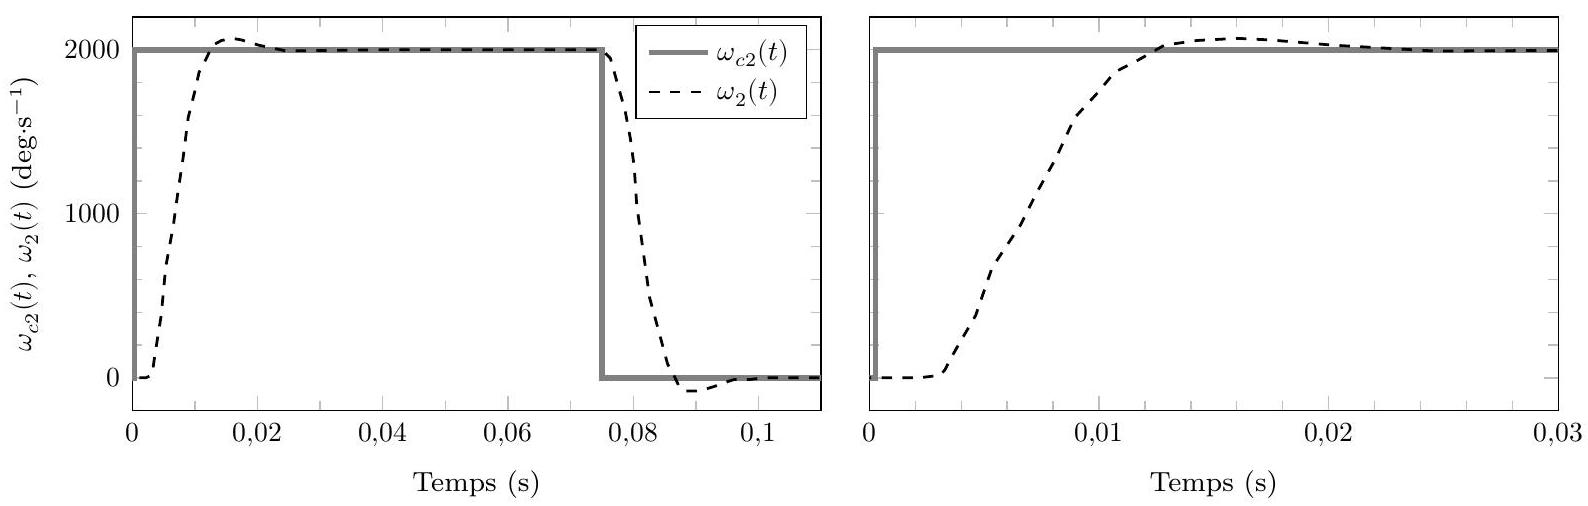
\includegraphics[width=\textwidth]{2023_07_26_54f5e859400a10e656ddg-05(1)}
%Figure 7 
\caption{\label{fig_ccspsi2022:07}Réponse expérimentale de l'étrier et consigne associée (à droite, zoom sur le régime transitoire)}
\end{figure}

Les transformées de Laplace de $\omega_{2}(t), \omega_{c 2}(t), \theta_{2}(t)$ et $c_{x}(t)$ sont notées $\Omega_{2}(p), \Omega_{c 2}(p), \theta_{2}(p)$ et $C_{x}(p)$.

%Q 10. 
\question{\label{q:10}Vérifier que la condition de réactivité énoncée ci-dessus est respectée. Justifier que la fonction de transfert de l'étrier (2) $H_{2}(p)=\frac{\Omega_{2}(p)}{\Omega_{c 2}(p)}$ peut alors être approchée par un gain statique $K_{2}$ de valeur à préciser. Il faut s'assurer que la position $\theta_{2}$ de l'étrier (2) ne s'éloigne pas trop de sa position de référence $\theta_{2}^{*}=0$. Le non-respect de cette condition, appelé dérive de l'étrier, génère un moment parasite $M_{01}$ responsable d'un déplacement du point $P$ selon $\vec{x}_{1}$.}

\subsection{\label{sec:II.B} Réglage du correcteur de la chaine d'asservissement de l'étrier}
La figure \ref{fig_ccspsi2022:08} montre la boucle d'asservissement sur la position $\theta_{2}(t) . C(p)$ est la fonction de transfert d'un correcteur appelé correcteur d'étrier. La dérive de l'étrier sera évitée si $\lim\limits_{t \rightarrow+\infty} \theta_{2}(t)=0$ lorsque la commande de l'étrier $U(p)$ est un échelon.

\begin{figure}[!h]
\centering
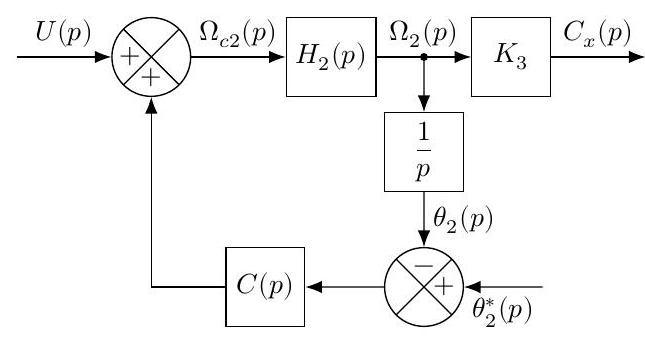
\includegraphics[width=.5\textwidth]{2023_07_26_54f5e859400a10e656ddg-05}
%Figure 8 
\caption{\label{fig_ccspsi2022:08}Asservissement de l'étrier}
\end{figure}

Les deux cas suivants sont envisagés :

\begin{itemize}
  \item avec une correction proportionnelle : $C(p)=K_{10}$;
  \item avec une correction proportionnelle-intégrale : $C(p)=K_{10}+\frac{K_{11}}{p}$.
\end{itemize}


%Q 11. 
\question{\label{q:11}Exprimer sous forme canonique la fonction de transfert $H_{\theta_{2}}(p)=\frac{\theta_{2}(p)}{U(p)}$ en fonction de $C(p)$ et $K_{2}$. Après avoir déterminé $\lim\limits_{t \rightarrow+\infty} \theta_{2}(t)$ lorsque $U(p)$ est un échelon unitaire dans les deux cas cités précédemment, justifier la pertinence d'une correction proportionnelle-intégrale au regard de la problématique de la dérive de l'étrier. Dans la suite de l'étude, le correcteur adopté est $C(p)=K_{10}+\frac{K_{11}}{p}$. L'effet gyroscopique $c_{x}(t)$ est lié à la vitesse de rotation $\omega_{2}(t)$ et la consigne $\theta_{2}^{*}(t)$ est maintenue à 0 pour éviter la dérive de l'étrier. La fonction de transfert utilisée pour modéliser le comportement de l'étrier (2) est notée $H_{m}(p)=\frac{\Omega_{2}(p)}{U(p)}$.}

%Q 12. 
\question{\label{q:12}Exprimer sous forme canonique la fonction de transfert $H_{m}(p)$ en fonction de $K_{2}, K_{10}$ et $K_{11}$.}

Le calcul des gains $K_{10}$ et $K_{11}$ doit répondre aux deux exigences suivantes: permettre d'éviter la dérive de l'étrier (2) et ne pas ralentir le système, d'où le choix d'une fonction de transfert $H_{m}(p)$ caractérisée par un amortissement $\xi_{m}=0,37$ et une pulsation propre $\omega_{m}=2,45 \mathrm{rad} \cdot \mathrm{s}^{-1}$.

%Q 13.
\question{\label{q:13} Déterminer les valeurs numériques de $K_{10}$ et $K_{11}$ au regard de ces exigences.}

%La rotation du stabilisateur (1) étudiée en partie \ref{sec:I} n'est pas prise en compte figure \ref{fig_ccspsi2022:6}. Il est indispensable de considérer la flexibilité de l'attache reconfigurable utilisée pour lier le stabilisateur (1) à la table d'opération (0).

\subsection{\label{sec:II.C} Comportement dynamique du stabilisateur}



Dans la modélisation retenue (figure \ref{fig_ccspsi2022:09}), une liaison pivot non parfaite permet de représenter la flexibilité de l'attache reconfigurable. La table d'opération (0) est supposée fixe et le référentiel $\mathcal{R}_{0}\left(O_{0}, \vec{x}_{0}, \vec{y}_{0}, \vec{z}_{0}\right)$ lié à la table (0) est galiléen. Au stabilisateur (1) est associé le repère $\mathcal{R}_{1}\left(O_{0}, \vec{x}_{0}=\vec{x}_{1}, \vec{y}_{1}, \vec{z}_{1}\right)$ avec $\theta_{1}=\left(\vec{y}_{0}, \vec{y}_{1}\right)=\left(\vec{z}_{0}, \vec{z}_{1}\right)$. Le point $P$ tel que $O_{0} P=L$ représente le bout du stabilisateur (1) en contact avec la zone à opérer.

\begin{figure}[!h]
\centering
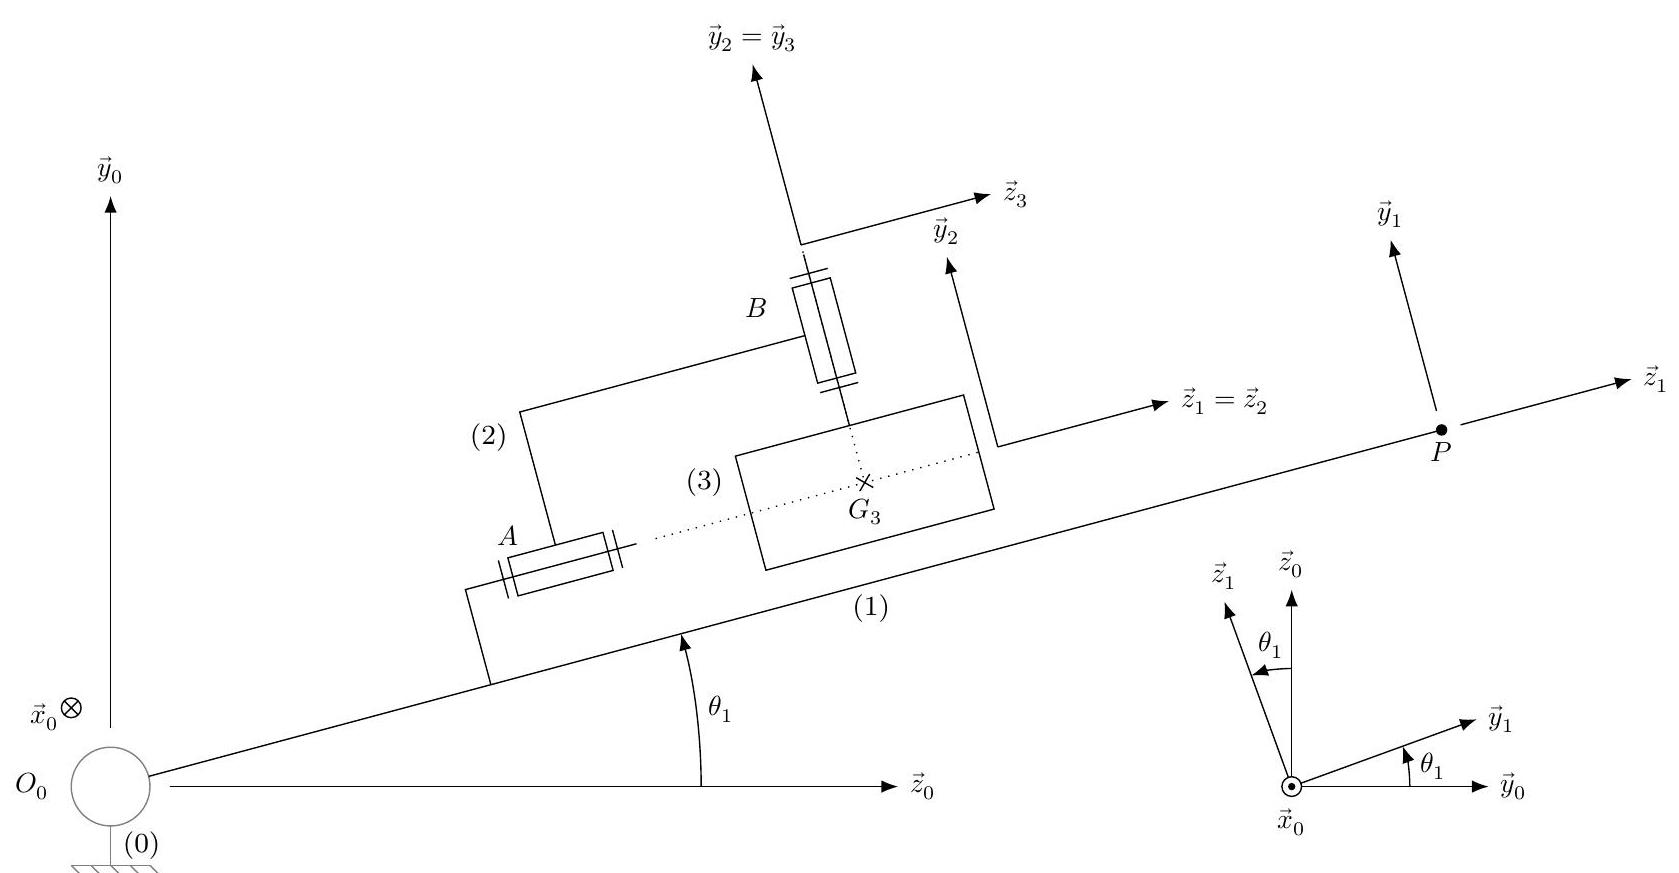
\includegraphics[width=.7\textwidth]{2023_07_26_54f5e859400a10e656ddg-06}
%Figure 9 
\caption{\label{fig_ccspsi2022:09}Modèle cinématique du système GyroLock (représenté pour $\theta_{2}=\theta_{3}=0$)}
\end{figure}

%
%\subsection*{Paramétrage, notations et hypothèses}
%\begin{itemize}
%  \item La liaison pivot d'axe $\left(O_{0}, \vec{x}_{0}\right)$ entre les solides (0) et (1) possède une raideur $k$ et un coefficient de frottement visqueux $f$, d'où $\vec{M}\left(O_{0}, 0 \rightarrow 1\right) \cdot \vec{x}_{0}=-\left(k \theta_{1}+f \dot{\theta}_{1}\right)$;
%
%  \item les autres liaisons sont supposées parfaites ;
%
%  \item l'action du cœur sur le stabilisateur (1) est modélisée par $\left\{\mathcal{T}_{c \rightarrow 1}\right\}=\left\{\begin{array}{c}f_{c} \vec{y}_{1} \\ \overrightarrow{0}\end{array}\right\}_{P}$;
%
%\item seul le déplacement vertical du point $P$ est pris en compte. On note $y(t)=-\overrightarrow{O_{0} P} \cdot \vec{y}_{0}$;
%
%\item  le stabilisateur (1) est de masse $m_{1}$ et possède un centre d'inertie $G_{1}$ tel que $\overrightarrow{O_{0} G_{1}}=L_{G_{1}} \vec{z}_{1}$ et l'opérateur d'inertie est $\mathcal{J}\left(G_{1}, 1\right)=\left[\begin{array}{ccc}A_{1} & 0 & 0 \\ 0 & A_{1} & 0 \\ 0 & 0 & C_{1}\end{array}\right]_{\mathcal{B}_{1}} ;$
%
%  \item la masse et l'inertie de l'étrier (2) sont négligeables ;
%
%  \item la toupie (3) est de masse $m_{3}$ et possède un centre d'inertie $G_{3}$ tel que $\overrightarrow{O_{0} G_{3}}=L_{G_{3}} \vec{z}_{1}+H_{G_{3}} \vec{y}_{1}$;
%
%  \item les figures de changement de base sont données figures 6 et 9 ;
%
%  \item les actions mécaniques dues à la pesanteur sont négligées devant les effets dynamiques. Q 14. Sans détailler les calculs, donner la méthode permettant de déterminer la loi de mouvement du stabilisateur (équation différentielle en $\theta_{1}(t)$ ). L'ensemble isolé, l'inventaire des actions mécaniques extérieures, le théorème utilisé et sa projection scalaire sont à préciser clairement.
%
%\end{itemize}
%
%%Q 15. 
%\question{\label{q:15}Exprimer $\vec{\delta}\left(O_{0}, 1 / 0\right) \cdot \vec{x}_{0}$, la projection sur $\vec{x}_{0}$ du moment dynamique au point $O_{0}$ du solide (1) en mouvement dans le référentiel $\mathcal{R}_{0}$.}
%
%%Q 16. 
%\question{\label{q:16}Exprimer littéralement la vitesse $\vec{V}\left(G_{3}, 3 / 0\right)$ dans la base $\mathcal{B}_{1}$, puis l'accélération $\vec{\Gamma}\left(G_{3}, 3 / 0\right)$ dans la base $\mathcal{B}_{1}$.}
%
%%Q 17. 
%\question{\label{q:17}En conservant les conditions de fonctionnement issues de la partie \ref{sec:II.A} $\left(\ddot{\theta}_{2} \approx 0, \theta_{2} \approx 0\right.$ et $\dot{\theta}_{3}=\omega_{3}$ constante), il est possible de montrer que $\vec{\delta}\left(G_{3}, 3 / 0\right) \cdot \vec{x}_{0}=A_{3} \ddot{\theta}_{1}-c_{x}(t)$ avec $c_{x}(t)=B_{3} \omega_{3} \dot{\theta}_{2}$ (résultat admis sans démonstration). En déduire $\vec{\delta}\left(O_{0}, 3 / 0\right) \cdot \vec{x}_{0}$, en fonction de $A_{3}, c_{x}(t), m_{3}, L_{G_{3}}, H_{G_{3}}$ et $\ddot{\theta}_{1}(t)$.}

%Q 18. 
%\question{\label{q:18}Exprimer $J_{x}$ en fonction de $A_{1}, A_{3}, m_{1}, m_{3}, L_{G_{1}}, L_{G_{3}}$ et $H_{G_{3}}$ permettant d'écrire la loi de mouvement du stabilisateur (1) sous la forme suivante :}


La loi de mouvement du stabilisateur (1) peut s'écrire sous la forme suivante :
$$
J_{x} \ddot{\theta}_{1}(t)+f \dot{\theta}_{1}(t)+k \theta_{1}(t)=c_{x}(t)-L f_{c}(t)
$$

En supposant que $\theta_{1}$ reste proche de 0, la relation $y(t)=L \theta_{1}(t)$ sera utilisée.

Les transformées de Laplace de $y(t), c_{x}(t)$ et $f_{c}(t)$ sont notées $Y(p), C_{x}(p)$ et $F_{c}(p)$.

%Q 19. 
\question{\label{q:19}En déduire les expressions littérales des fonctions de transfert $H_{\text {pert }}(p)$ et $H_{1}(p)$ du schéma-blocs figure \ref{fig_ccspsi2022:10} en fonction de $L, J_{x}, f$ et $k$.}


\begin{figure}[!h]
\centering
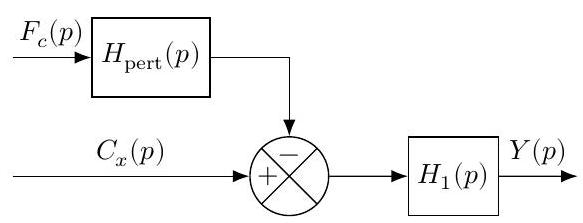
\includegraphics[width=.4\textwidth]{2023_07_26_54f5e859400a10e656ddg-07}
%Figure 10 
\caption{\label{fig_ccspsi2022:10}Schéma bloc du stabilisateur (1)}
\end{figure}

On rappelle que $L=0,3 \mathrm{~m}$ et les valeurs retenues pour $J_{x}, f$ et $k$ sont :

\begin{itemize}
  \item $J_{x}=1,14 \times 10^{-2} \mathrm{~kg} \cdot \mathrm{m}^{2}$;

  \item $-f=64 \times 10^{-3} \mathrm{~N} \cdot \mathrm{m} \cdot \mathrm{s} \cdot \mathrm{rad}^{-1}$;

  \item $-k=95 \mathrm{~N} \cdot \mathrm{m} \cdot \mathrm{rad}^{-1}$.
\end{itemize}

%Q 20. 
\question{\label{q:20}Écrire $H_{1}(p)$ sous forme canonique, puis calculer les valeurs de ses paramètres caractéristiques : gain statique $K_{1}$, amortissement $\xi_{1}$ et pulsation propre $\omega_{1}$. Commenter le comportement associé (fréquentiel ou temporel).}

\section{Réglage de la loi de commande du stabilisateur}
\begin{obj}
Régler une loi de commande permettant de respecter les exigences figure \ref{fig_ccspsi2022:03}.
\end{obj}

Le faible amortissement de la fonction de transfert $H_{1}(p)$ et la rapidité du système imposent la mise en place de deux boucles d'asservissement :
\begin{itemize}
 \item  un asservissement en vitesse de la vitesse $v(t)=\dot{y}(t)$;
  \item un asservissement en position de la position $y(t)$.
\end{itemize}

Le schéma-blocs global du système est donné figure \ref{fig_ccspsi2022:11}, où :

\begin{itemize}
  \item $H_{m}(p)$ est la fonction de transfert de l'étrier asservi ;

  \item $Y^{*}(p)$ est une consigne virtuelle de valeur nulle ;

  \item $K_{p}$ et $K_{v}$ sont deux gains à déterminer.

\end{itemize}


\begin{figure}[!h]
\centering
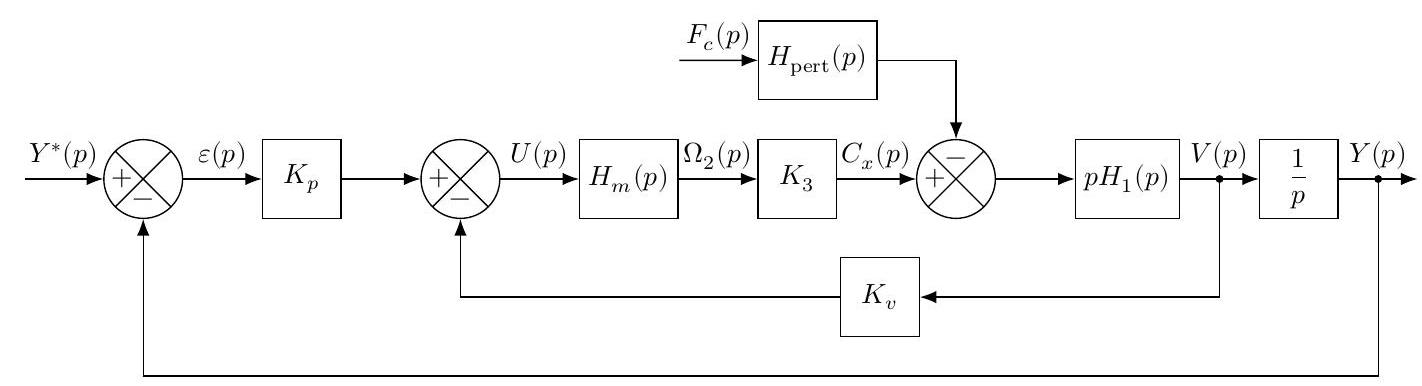
\includegraphics[width=\textwidth]{2023_07_26_54f5e859400a10e656ddg-07(1)}
%Figure 11 
\caption{\label{fig_ccspsi2022:11}Schéma-blocs global du système GyroLock}
\end{figure}

\section{\label{sec:III.A} Valeur maximale de $K_{p}$}
%Q 21.

\question{\label{q:21}Exprimer la fonction de transfert en boucle ouverte $H_{\mathrm{BO}}(p)=\frac{Y(p)}{\varepsilon(p)}$ en fonction de $K_{p}, K_{3}, K_{v}$, $H_{m}(p)$ et $H_{1}(p)$.}

Un premier choix de conception de la commande a conduit à imposer $K_{v}=15$. Le diagramme de Bode de $H_{\mathrm{BO}}(p)$ pour $K_{p}=1$ est donné figure \ref{fig_ccspsi2022:12}. Pour ce tracé, la fonction de transfert $H_{2}(p)=\frac{\omega_{0}^{2}}{p^{2}+2 \xi \omega_{0} p+\omega_{0}^{2}}$ non simplifiée est utilisée, avec $\omega_{0}=200 \mathrm{rad} \cdot \mathrm{s}^{-1}, \xi=0,7$, et les valeurs de $K_{10}, K_{11}$ sont celles obtenues avec le modèle simplifié de la question~\ref{q:13}.


\begin{figure}[!h]
\centering
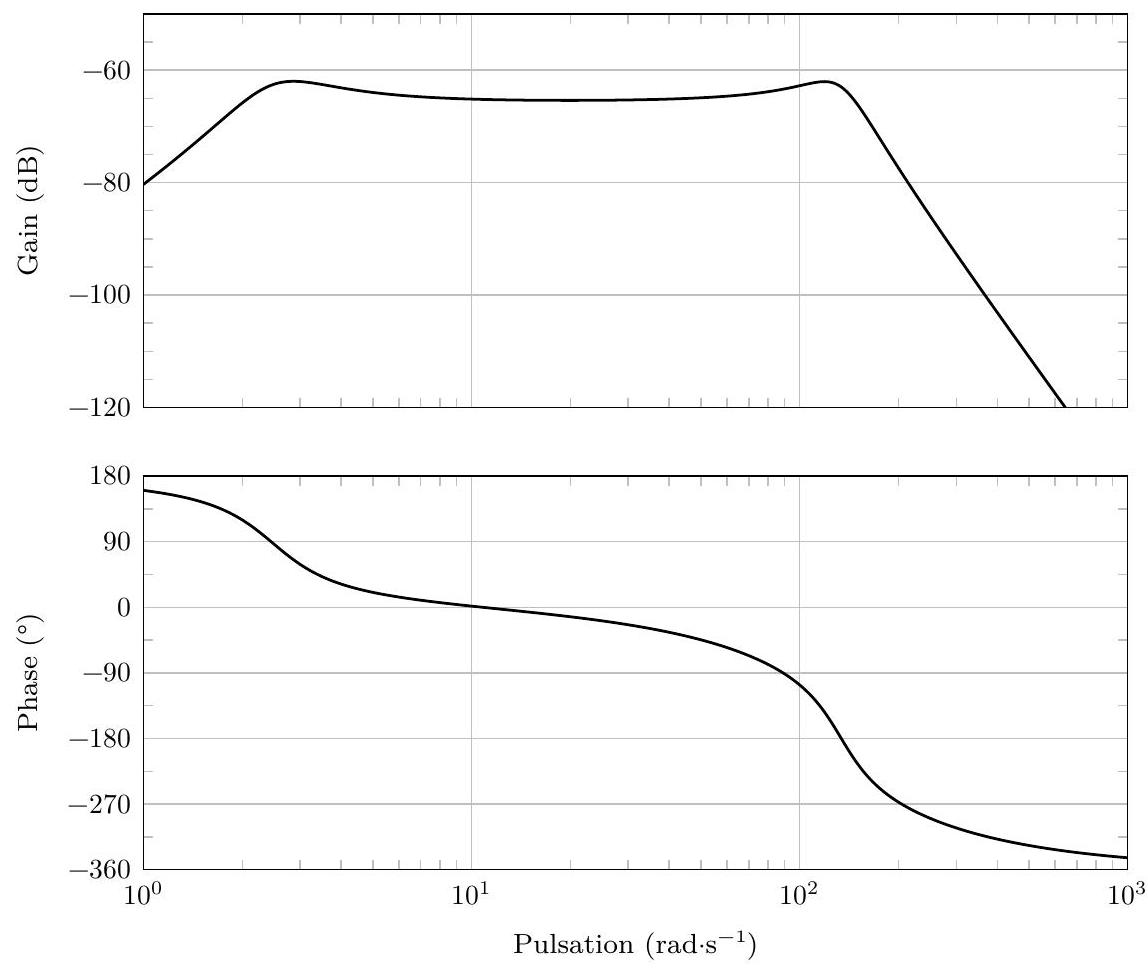
\includegraphics[width=.9\textwidth]{2023_07_26_54f5e859400a10e656ddg-08(1)}
%Figure 12 
\caption{\label{fig_ccspsi2022:12}Diagramme de Bode de la boucle ouverte avec $K_{p}=1$}
\end{figure}

%Q 22. 
\question{\label{q:22}À partir de la figure \ref{fig_ccspsi2022:12}, donner la valeur maximale de $K_{p}$ telle que le système soit stable en boucle fermée.}

\subsection{\label{sec:III.B} Vérification de la valeur de $K_{p}$}
%Q 23. 
\question{\label{q:23}Déterminer la valeur maximale $G_{\max }$ du gain de la fonction de transfert $\left|\frac{Y(j \omega)}{F_{c}(j \omega)}\right|$ qui permet de garantir le respect des exigences du diagramme figure \ref{fig_ccspsi2022:03}.}

La figure \ref{fig_ccspsi2022:13} donne, en fonction de la valeur de $K_{p}$, la valeur maximale du gain $\left|\frac{Y(j \omega)}{F_{c}(j \omega)}\right|$ pour les fréquences cardiaques précisées par l'exigence 1.1.1 de la figure \ref{fig_ccspsi2022:03}.


\begin{figure}[!h]
\centering
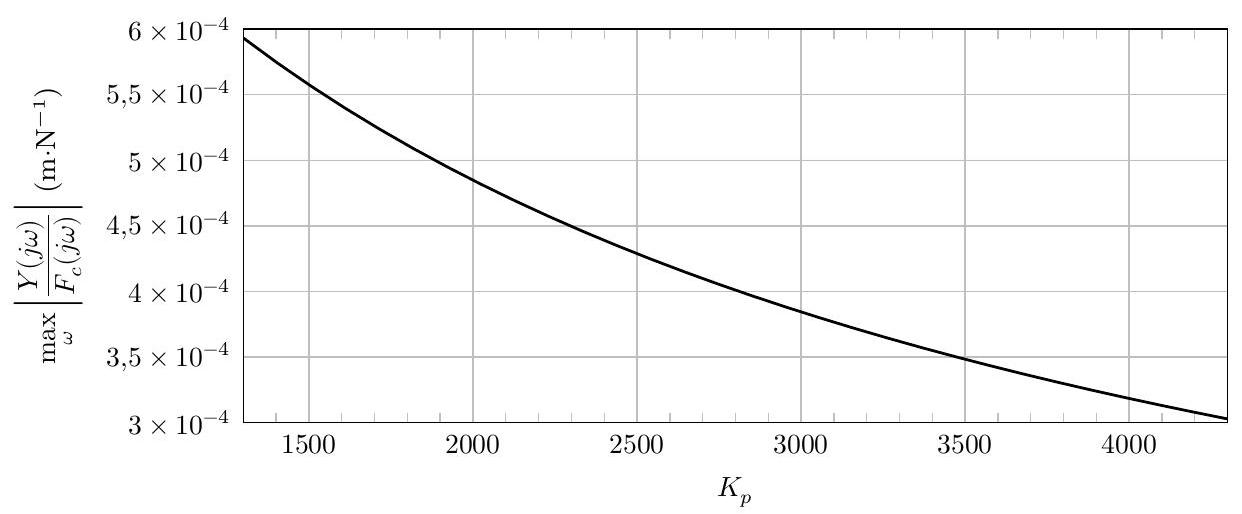
\includegraphics[width=.9\textwidth]{2023_07_26_54f5e859400a10e656ddg-08}
%Figure 13 
\caption{\label{fig_ccspsi2022:13}Gain maximal de la réponse fréquentielle de la fonction de transfert $\frac{Y(p)}{F_{c}(p)}$ en fonction de $K_{p}$}
\end{figure}

\question{À partir de la figure \ref{fig_ccspsi2022:13}, déterminer la valeur minimale de $K_{p}$ permettant de respecter l'exigence~1.1. Vérifier la cohérence de cette valeur avec celle trouvée à la question \ref{q:22} .}

\subsection{\label{sec:III.C} Amélioration des performances par compensation de l'effort cardiaque}
Une solution pour améliorer la commande du système serait de compenser l'effet de l'effort cardiaque en complétant la commande $U(p)$ de l'étrier par une anticipation du type $C_{a}(p) F_{c}(p)$ avec $C_{a}(p)$ un correcteur à déterminer. Cependant, il n'est pas envisageable de mesurer l'effort cardiaque du patient. L'utilisation d'un observateur permet d'obtenir une estimation $\hat{f}_{c}(t)$ à partir des mesures de $y(t)$ et $v(t)=\dot{y}(t)$ (issues d'un accéléromètre lié au support du GyroLock). Cette structure de commande peut être représentée par le schéma-blocs figure \ref{fig_ccspsi2022:14}.

\begin{figure}[!h]
\centering
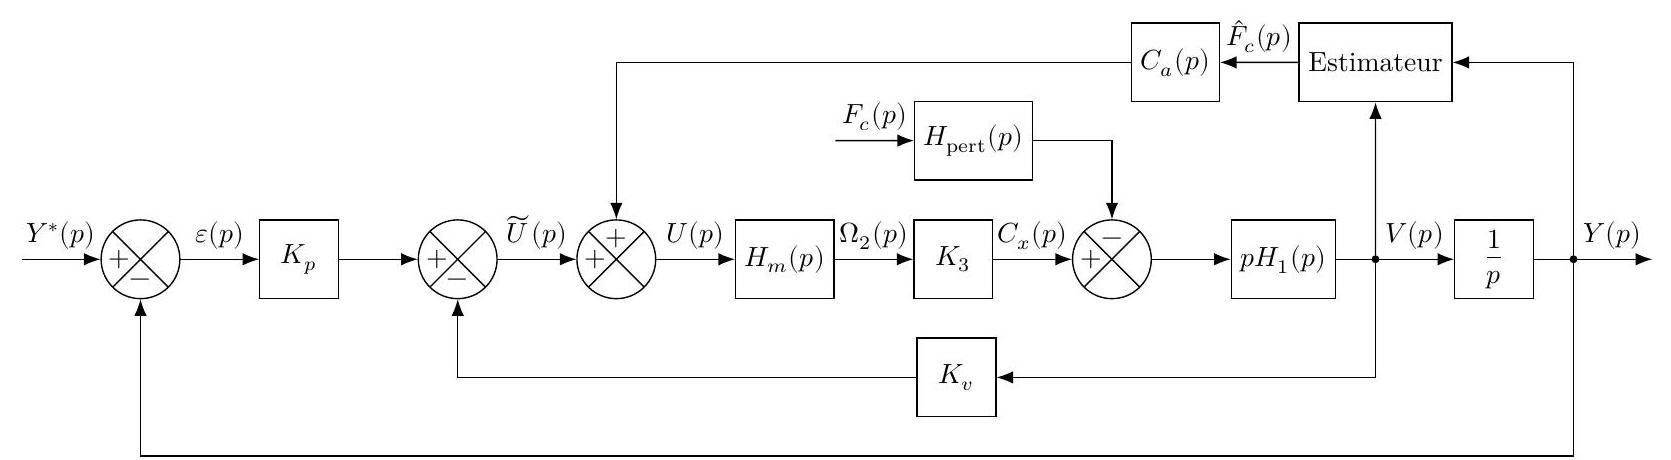
\includegraphics[width=\textwidth]{2023_07_26_54f5e859400a10e656ddg-09(1)}
\caption{\label{fig_ccspsi2022:14}Schéma bloc de la commande avec estimation et compensation de l'effort cardiaque}
\end{figure}

En première approximation :
\begin{itemize}
\item l'estimateur est modélisé par un premier ordre de constante de temps $\tau=5 \mathrm{~ms}$ et de gain unitaire ;
  \item la fonction de transfert $H_{m}(p)$ est modélisée par la forme approchée $H_{m}(p)=\frac{p^{2}}{p^{2}+2 \xi_{m} \omega_{m} p+\omega_{m}^{2}}$.
\end{itemize}

La consigne virtuelle $Y^{*}(p)$ étant nulle, la structure de commande peut alors être représentée par le schéma-blocs figure~\ref{fig_ccspsi2022:15}.

\begin{figure}[!h]
\centering
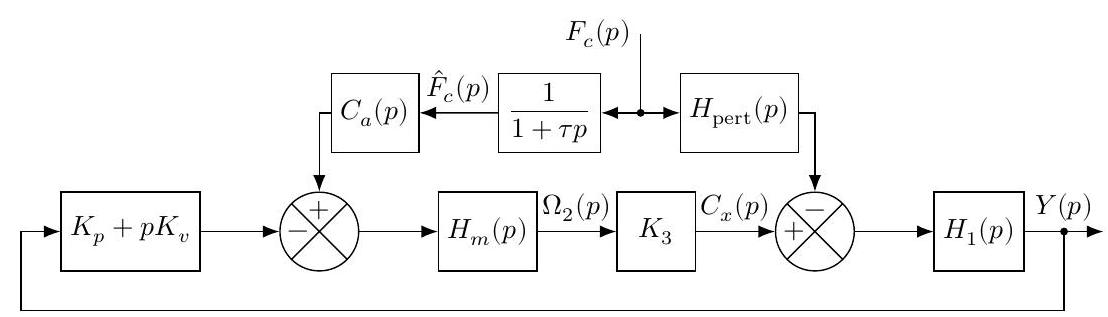
\includegraphics[width=\textwidth]{2023_07_26_54f5e859400a10e656ddg-09}
%Figure 15 
\caption{\label{fig_ccspsi2022:15}Schéma bloc de la commande}
\end{figure}

%Q 25. 
\question{\label{q:25}Exprimer la fonction de transfert $H_{F_{c}}^{\text {est }}(p)=\frac{Y(p)}{F_{c}(p)}$ en fonction de $K_{p}, K_{v}, K_{3}, H_{\text {pert }}(p), \tau, C_{a}(p)$, $H_{m}(p)$ et $H_{1}(p)$.}

%Q 26. 
\question{\label{q:26}En déduire l'expression de $C_{a}(p)$ permettant de rejeter la perturbation $F_{c}(p)$, en fonction de $H_{\text {pert }}(p)$, $\tau, K_{3}$ et $H_{m}(p)$, puis en fonction de $L, \tau, \xi_{m}, \omega_{m}$ et $K_{3}$.}

%Q 27.
\question{\label{q:27}Analyser les problèmes éventuels liés à la réalisation de ce correcteur. Conclure sur la possibilité de son implantation dans le système de commande.}

Le diagramme de Bode associé au correcteur $C_{a}(p)$, exprimé question \ref{q:26}, est donné figure \ref{fig_ccspsi2022:16}. Pour des raisons de simplification, une forme approchée du correcteur $C_{a}(p)$ doit être déterminée.

%Q 28. 
\question{\label{q:28}À partir de la figure \ref{fig_ccspsi2022:16} et de l'exigence 1.1.1, justifier qu'une approximation de $C_{a}(p)$ sous la forme d'un gain proportionnel $\widetilde{C_{a}}(p)=K_{a}$ est suffisante. Déterminer la valeur numérique de $K_{a}$.}

La figure \ref{fig_ccspsi2022:17} montre les gains des réponses fréquentielles de l'effort de perturbation $f_{c}$ vers la position $y$ pour différents cas : en boucle ouverte, en boucle fermée avec la structure de commande définie dans cette étude sans anticipation et en boucle fermée avec anticipation.

L'exploitation des modèles conduit en simulation numérique aux évolutions temporelles de $y(t)$ et de $\theta_{2}(t)$ (obtenues avec $K_{p}=500$ et une valeur de $K_{a}$ proche de celle déterminée à la question \ref{q:28}) présentées figure \ref{fig_ccspsi2022:18}. 

%Q 29. 
\question{\label{q:29}Analyser les courbes des figures \ref{fig_ccspsi2022:17} et \ref{fig_ccspsi2022:18} et les commenter en considérant des critères (non exhaustifs) comme les coefficients d'amortissement obtenus, les niveaux d'atténuation de la perturbation d'effort au regard du cahier des charges défini figure \ref{fig_ccspsi2022:03}, la cohérence des résultats montrés par les figures \ref{fig_ccspsi2022:17} et \ref{fig_ccspsi2022:18}, etc.
Conclure sur la capacité du système GyroLock, tel qu'il a été modélisé dans cette étude, à maintenir la zone à opérer lors d'une opération à cœur battant.}

\begin{figure}[!h]
\centering
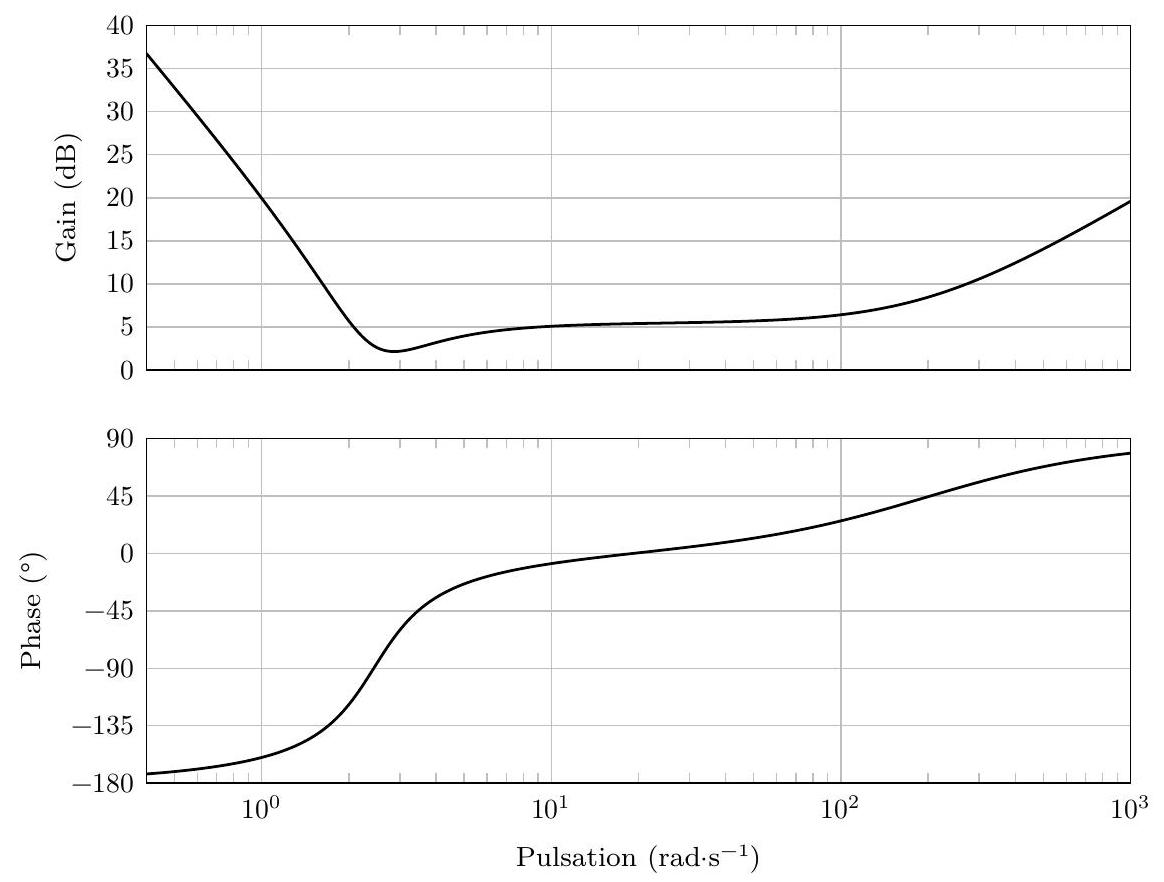
\includegraphics[width=.9\textwidth]{2023_07_26_54f5e859400a10e656ddg-10(1)}
%Figure 16 
\caption{\label{fig_ccspsi2022:16}Diagramme de Bode du correcteur $C_{a}(p)$}
\end{figure}


\begin{figure}[!h]
\centering
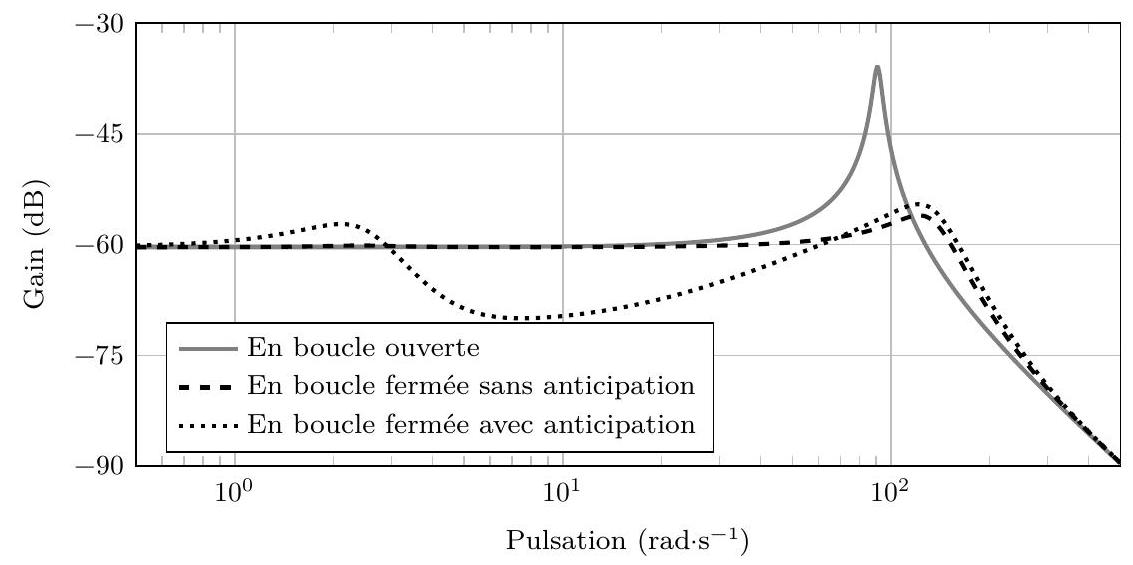
\includegraphics[width=.9\textwidth]{2023_07_26_54f5e859400a10e656ddg-10(2)}
%Figure 17 
\caption{\label{fig_ccspsi2022:17}Réponses fréquentielles $\left|Y(j \omega) / F_{c}(j \omega)\right|$}
\end{figure}


\begin{figure}[!h]
\centering
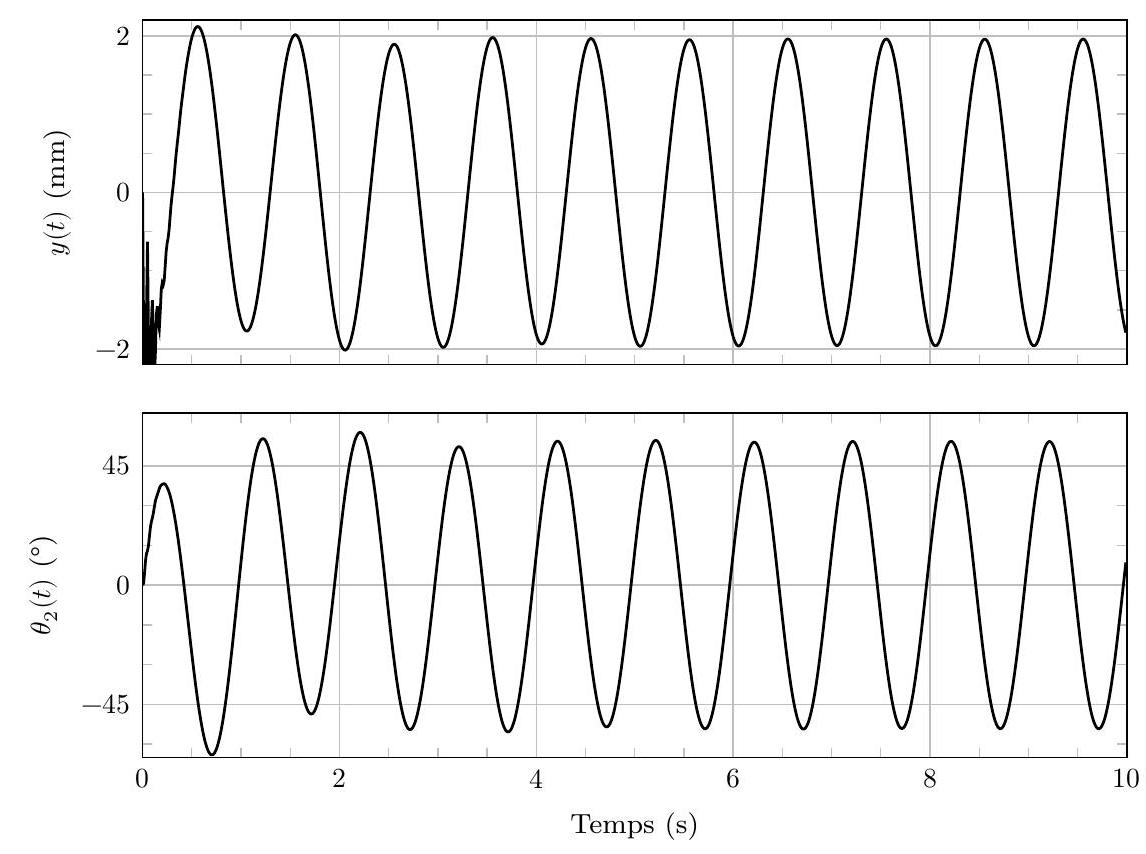
\includegraphics[width=.9\textwidth]{2023_07_26_54f5e859400a10e656ddg-10}
%Figure 18 
\caption{\label{fig_ccspsi2022:18}Évolutions temporelles de $y(t)$ et $\theta_{2}(t)$ avec estimation et compensation de $f_{c}(t)$}
\end{figure}

%\end{document}